\section{Example For Functional Analysis}
\label{sec:examples}

In the following section for four different systems the Functional Model will be implemented.
With the given Functional Model the problems of the system can be obtained.
Afterwards with the help of the various Matrices and the Principles solutions for these problems can be found.
For some optimizable functions a principle will be looked up in the matrix, which will be visible in the examples. 
Some functions will not be optimized on purpose, as this should help to figure out own ideas and solutions.

For the following examples always one implementation of a function is described.
The creation of the other functions in the example works analogously.

\subsection{Example Washing Machine}

The first examples describes the system of a washing machine. 
This example was used by Nikolai Shchedrin. 

First the important system components \textit{Washing Machine Drum} and \textit{Laundry} were defined as an component.
Furthermore the action \textit{Turn} is implemented.
With the two components the interaction \textit{Washing Machine Drum - Laundry} is created.

At point three, as mentioned before, the function \textit{CirculateLaundry} is created. 

In the next step the direction for the function is added. 
This is done, by defining the Subject-Action-Object triple \textit{Washingmachinedrum - Turn - Laundry}, with the interaction and the action.
In this case \textit{Washing Machine Drum} is the Subject and the \textit{Laundry} is the Object.
Afterwards this attached to the function.

In the final step we create the quality of the function. 
At this point the creator has to analyze the function and reason why this quality was chosen.
Here, the quality was chosen as a \textit{Useful Function}, as the turning of the laundry helps the cleaning.
Furthermore it is assumed that the washing machine works perfectly in this aspect.
Otherwise the function could have a harmful addition.
The quality is then added as another triple to the function.

At this point the function has all important triples. 
The function in figure \ref{fig:implementation_function_circulate_laundry} then represents one part of the Functional Model. 

\begin{figure}[H]
    \centering
    \begin{code}\tt
        ex:CirculateLaundry\\
        \> a tc:Function ;\\
        \> tc:SubjectActionObject ex:WashingmachinedrumTurnLaundry ;\\
        \> tc:QualityOfFunction tc:UsefulFunction ;\\
        \> skos:prefLabel "Ciruclate Laundry"@en .\\
    \end{code}
    \caption{Implementation Of The Function \textit{CirculateLaundry}}
    \label{fig:implementation_function_circulate_laundry}
\end{figure}

\subsection{Example Coffee}

The next example is mentioned in the book "Systematische  Innovationsmethoden".
The example describes the system of coffee interacting with a cup when poured into it.
A small part of the Functional Model is implemented as a RDF graph. 

At first the two components \textit{Cup} and \textit{Coffee} are implemented in \textit{ex} namespace.
With the two components the interaction \textit{CupCoffee} is created.
Afterwards the action \textit{Rest} is added.

With the components and action defined, the function \textit{Pollute}, which can be seen in figure \ref{fig:implementation_function_pollute} is created.
This describes that the coffee leaves residues at the cup. 

As before, the direction of the function is added with the Subject-Action-Object triple.
In this case this is named \textit{CupRestCoffee} and the Subject is the \textit{Coffee}. 

As the residue is a negative effect this would be a \textit{Harmful Function}.
Hence this function would be a starting point to find a Principles in the Matrix to solve this problem.

With the creation of further functions the Functional Model is fulfilled. 
At last all the functions with problems can be analyzed and a suitable Matrix Entry can be identified.
From there a Principle is chosen, which optimizes the function.

\begin{figure}[H]
    \centering
    \begin{code}\tt
        ex:Pollute\\
        \> a tc:Function ;\\
        \> tc:SubjectActionObject ex:CoffeeRestCup ;\\
        \> tc:QualityOfFunction tc:HarmfulFunction ;\\
        \> skos:prefLabel "Pollute"@en .\\
    \end{code}
    \caption{Implementation Of The Function \textit{Pollute}}
    \label{fig:implementation_function_pollute}
\end{figure}

\subsection{Example Car}

In the third example the system of a car is analyzed.
Hereby the function \textit{SitUncomfortable} is explained.

First of all the two components \textit{UncomfortableSeats} and \textit{Inmates} are created.
The action is in this case \textit{Touch} and the Subject-Action-Object triple will be \textit{InmatesTouchUncomfortableSeats}.
The \textit{Inmates} are the Subject as these are touching the seats.

The quality of the function is a \textit{Function Disadvantage}, as the inmates are able to sit, which is a positive or useful aspect. 

On the other hand the seats are uncomfortable for the inmates.
This can be harmful as the driver can be disturbed by this. 
Furthermore, as the feeling of a uncomfortable seat differs for each person, this function is bad controllable.
\begin{figure}[H]
    \centering
    \begin{code}\tt
        ex:SitUncomfortable\\
        \> a tc:Function ;\\
        \> tc:SubjectActionObject ex:InmatesTouchUncomfortableSeats ;\\
        \> tc:QualityOfFunction tc:FunctionDisadvantage ;\\
        \> skos:prefLabel "Uncomfortable Sitting"@en ;\\
        \> skos:Definition "By touching the occupants with the uncomfortable seats of\\
        \> \> the car, a useful function forms with disadvantages, since the occupants\\
        \> \> on the one hand can sit but only uncomfortably"@en .
    \end{code}
    \caption{Implementation Of The Function \textit{SitUncomfortable}}
    \label{fig:implementation_function_sit_uncomfortable}
\end{figure}

\subsection{Example Mechanical Computer Mouse}

The last example is taken from the book "Systematische  Innovationsmethoden".
Picture \ref{fig:functional_model_mechanical_computer_mouse} shows an overview over the Functional Model. 
This picture was created by the book authors \cite{KS}.
The different arrows represent different kind of qualities for the function.
The black arrows are Useful Functions, the red ones describe Harmful Functions and the dotted lines represent a Bad Controllable Function.

\begin{figure}[H]
    \centering
    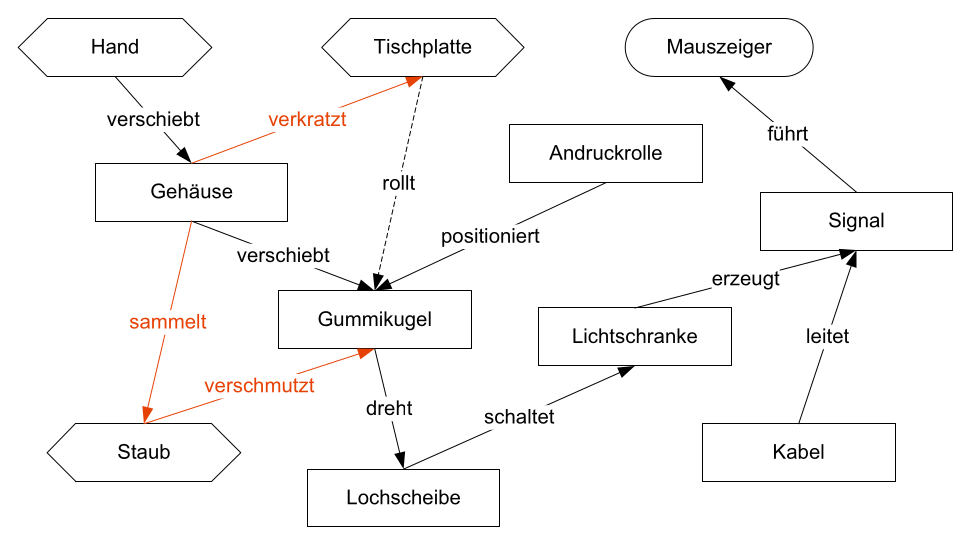
\includegraphics[scale=.6]{pictures/functional_model_mechanical_computer_mouse.png}
    \caption{Functional Model For A Mechanical Computer Mouse In German}
    \label{fig:functional_model_mechanical_computer_mouse}
\end{figure}

The implementation of the function \textit{Scratches} is going to be explained.
This describes the arrow from \textit{Case (Gehäuse)} to \textit{Tabletop (Tischplatte)}.

The interaction is therefore \textit{CaseTabletop} with the two components \textit{Case} and \textit{Tabletop}.
All of these are in the ex namespace as explained in section \ref{sec:conceptualisations}.

Furthermore the action \textit{Move} is defined. 
And with that the direction \textit{CaseMoveTabletop}, by the Subject-Action-Object triple created.

Finally the quality of the function is added.
The book defined this as a \textit{Harmful Function}.

As this is an Harmful Function an optimization is necessary. 
Therefore we define \textit{ScratchesParameter} which is a \textit{functionWithMatrixParameter} concept. 
Hence we have to choose the decreasing and increasing parameters.
As in this paper also the Matrix 2003 was implemented.
This is the one chosen to find a suitable principle.

As an increasing parameter \textit{Power} is chosen, because the moving of the mouse increases the working possibilities of the mouse. 
The decreasing parameter is \textit{Loss Of Material}, as the tabletop looses material during the moving of the mouse. 

With the chosen parameters the matrix entry can be obtained. 
In this case this would be \textit{$<$http://opendiscovery.org/rdf/Matrix/E.18.25$>$}. 

From there the principle \textit{tc:FlexibleCoversOrThinFilms} is picked.

This should lead to an optimization for the function.
Here it could be adding a layer between the tabletop and the mouse, like a mouse-pad. 
